\chapter{Conjuntos y \textit{piecewise maps} ordenados}

Una vez establecidos los conceptos necesarios, a continuación se presenta la estructura de los \textbf{conjuntos ordenados} y de los \textbf{\textit{piecewise maps} ordenados}. El objetivo es mostrar cómo cada una de estas entidades almacena, respectivamente, multi-intervalos y mapas, y de qué manera gestionan la información que permite mantener el orden dentro de cada una.

\section{Estructura y orden de conjunto ordenados}

Como se mencionó previamente en la subsección dedicada a los conjuntos ordenados densos, estos utilizaban el operador $<$ definido para los multi-intervalos para dotarse de orden. Los \textbf{conjuntos ordenados} utilizan el mismo criterio para dotarse de orden. Por lo tanto, la estructura de los conjuntos ordenados, denominados \texttt{OrderedSet}, incluye la siguiente variable miembro:

\begin{itemize}
  \item \texttt{pieces\_} (de tipo \textbf{MDIOrdSet}): representa el conjunto en si mismo.
\end{itemize}

Ahora bien, a diferencia de los conjuntos ordenados densos, que operaban sobre una única dimensión, los conjuntos ordenados trabajan sobre múltiples dimensiones. En consecuencia, el operador $<$ definido para el tipo \texttt{MD\_NAT} que se utiliza por debajo ya no se limita a una comparación tradicional entre valores numéricos, sino que ya trabaja a nivel dimensional como se mostró en el capitulo de conceptos previos.

Supóngase que se trabaja con multi-intervalos bidimensionales, donde cada uno posee su correspondiente mínimo. Sean entonces por ejemplo los siguientes tres multi-intervalos:

\begin{itemize}
    \item $mdi_1 =$ $|[2:1:2]\times[3:2:9]|$, con mínimo $(2,\ 3)$
    \item $mdi_2 =$ $|[1:1:2]\times[5:2:9]|$, con mínimo $(1,\ 5)$
    \item $mdi_3 =$ $|[2:1:2]\times[1:2:9]|$,con mínimo $(2,\ 1)$
\end{itemize}

Aplicando el criterio de orden basado en los mínimos, junto con el operador $<$ definido para los multi-intervalos, se obtiene el siguiente ordenamiento:

\begin{center}
\[
mdi_2 < mdi_3 < mdi_1
\]

ya que:

\[
(1,\ 5) < (2,\ 1) < (2,\ 3)
\]

Por lo tanto, el conjunto ordenado resultante será:

\[
\{mdi_2,\ mdi_3,\ mdi_1\}
\]
\end{center}


\section{Estructura y orden de \textit{piecewise maps} ordenados}

Ahora es el turno de los \textbf{\textit{piecewise maps} ordenados}. A diferencia de los conjuntos ordenados, no se disponía de una implementación previa que ofreciera una estructura ordenada de ninguna índole capaz de brindar pistas de como desarrollar el criterio de orden. En consecuencia, fue necesario desarrollar dicho criterio desde cero.

Inicialmente, los piecewise maps ordenados deben contar con una variable miembro que contenga los mapas que se desean almacenar. Esta variable se denominará \texttt{pieces\_}, aunque por el momento no se le asignará un tipo concreto, ya que primero es necesario definir el criterio de orden.

El objetivo es construir un criterio de orden que permita reutilizar y aprovechar los conceptos desarrollados para optimizar los conjuntos ordenados, aun cuando ahora se trabaja con mapas. Recordemos que un \texttt{Map} está definido por las siguientes dos componentes:

\begin{itemize}
  \item Un conjunto dominio;
  \item Una colección de expresiones lineales.
\end{itemize}

Se decidió tomar como base del criterio de orden a los conjuntos dominio, ya que estos están estrechamente relacionados con los multi-intervalos y puede ayudar a cumplir objetivo planteado anteriormente. En cambio, las expresiones lineales no aportan ninguna ventaja aparente, por lo cual son descartadas para gestionar el orden dentro de los \textit{piecewise maps} ordenados.

Definido el elemento sobre el cual se va a basar el orden, corresponde establecer cuándo un mapa se considera estrictamente menor que otro:

\begin{center}
Sean $m_1 = \{ dom_1 \rightarrow exps_1 \}$ y $m_2 = \{ dom_2 \rightarrow exps_2 \}$ dos mapas arbitrarios, es decir, objetos de tipo \texttt{Map}. \\
Entonces, se define que $m_1 < m_2$ si y solo si $minPer_1 < minPer_2$, \\
donde la comparación se realiza con el operador $<$ de los naturales multi-dimensionales o \texttt{MD\_NAT}, y $minPer_1$ y $minPer_2$ son los mínimos perimetrales de $dom_1$ y $dom_2$, respectivamente.
\end{center}

Ahora bien, el mínimo perimetral se define de la siguiente manera:

\begin{center}
Sea $m = (m_0, m_1, \dots, m_{n-1})$ un natural multi-dimensional o \texttt{MD\_NAT}, y sea $C$ un conjunto. \\
Entonces, $m$ es el \textbf{mínimo perimetral} de $C$ si para todo $j \in \{0, \dots, n-1\}$ se cumple:

\begin{itemize}
    \item $m_j = x_j$, donde $x_j$ es la componente $j$ del mínimo de algún multi-intervalo de $C$;
    \item y $m_j \leq x_j$, donde $x_j$ es la componente $j$ para todos los mínimos de los multi-intervalos de $C$.
\end{itemize}
\end{center}

Teniendo todo esto presente, y dado que los conjuntos no implementan ningún método que permita calcular el mínimo perimetral, ya que no es una operación inherente a su naturaleza, la idea será generar una operación adicional para calcular dicho mínimo, realizar esa operación una única vez (ya que implica recorrer todos los mínimos de un conjunto debido a la definición del mínimo perimetral), y almacenarlo junto con su mapa correspondiente. 

En consecuencia, la variable \texttt{pieces\_} tendrá la siguiente forma:

\[
\texttt{pieces\_} = \ll (m_0,\ minPer_0),\ (m_1,\ minPer_1),\ \dots,\ (m_{k-1},\ minPer_{k-1}) \gg
\]

donde para todo $i, j \in \{0,\dots,k-1\}$ con $i < j$, se cumple que $m_i < m_j$, es decir, $minPer_i < minPer_j$.

Con esto, el orden dentro de un \textit{piecewise map} ordenado queda definido. Sin embargo, esto no es suficiente para aprovechar por completo los conceptos utilizados para optimizar los conjuntos ordenados. Para ello, es necesario definir también el concepto de \textbf{máximo perimetral}:

\begin{center}
Sea $m = (m_0, m_1, \dots, m_{n-1})$ un elemento de tipo \texttt{MD\_NAT}, y sea $C$ un conjunto. \\
Entonces, $m$ es el \textbf{máximo perimetral} de $C$ si para todo $j \in \{0, \dots, n-1\}$ se cumple:

\begin{itemize}
    \item $m_j = x_j$, donde $x_j$ es la componente $j$ del máximo de algún multi-intervalo de $C$;
    \item y $m_j \geq x_j$, donde $x_j$ es la componente $j$ para todos los máximos de los multi-intervalos de $C$.
\end{itemize}
\end{center}

Esta información también debe ser almacenada, tal como se hizo con el mínimo perimetral. Por lo tanto, la variable \texttt{pieces\_} tendrá ahora la siguiente estructura extendida:


\begin{align*}
\texttt{pieces} = \ll \, 
  & (m_0,\ (\texttt{minPer}_0,\ \texttt{maxPer}_0)), \\
  & (m_1,\ (\texttt{minPer}_1,\ \texttt{maxPer}_1)), \\
  & \dots, \\
  & (m_{k-1},\ (\texttt{minPer}_{k-1},\ \texttt{maxPer}_{k-1})) \,\gg
\end{align*}



Este concepto funciona como contraparte del mínimo perimetral y permite interpretar el conjunto dominio de un mapa como si fuera un único multi-intervalo definido por su mínimo y su máximo perimetral. En la Figura~\ref{fig:minmaxPer1} se muestra un ejemplo de esta interpretación de manera gráfica, donde el multi-intervalo que se menciono antes esta marcado en linea punteada. Se hará mucho mas incapie en este concepto al llegar al capitulo de optimizaciones de \textit{piecewise maps} ordenados.

\begin{figure}[ht]
  \centering
  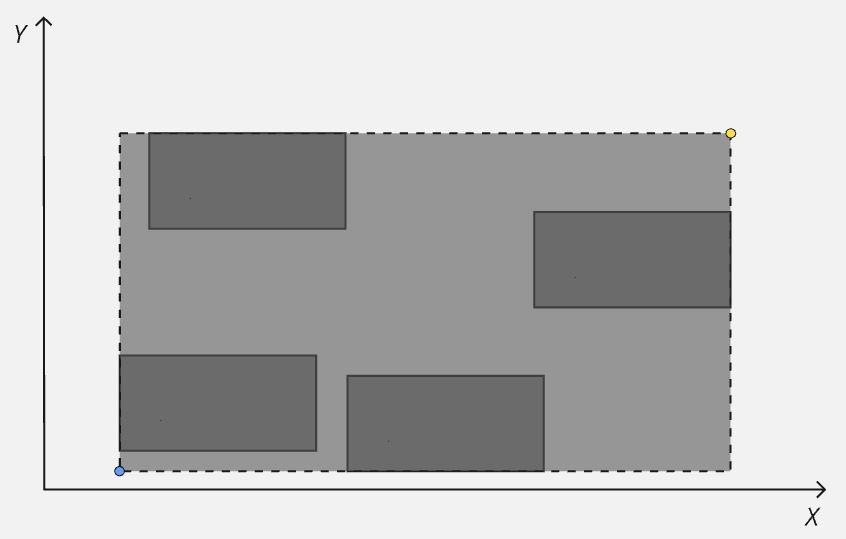
\includegraphics[width=0.6\textwidth]{figures/Orden/image.png}
  \caption{Representación gráfica del conjunto dominio de un mapa con 4 multi-intervalos, mas el marcado del mínimo y máximo perimetral en azul y amarillo resp.}
  \label{fig:minmaxPer1}
\end{figure}


Con toda esta información ya se puede declarar formalmente cómo está constituida la variable \texttt{pieces\_} para los \textit{piecewise maps} ordenados, denominados como \texttt{OrdPWMap}:

\begin{itemize}
  \item \texttt{pieces} (de tipo \textbf{OrdMapCollection}): 
  representa la colección ordenada de mapas junto con la información perimetral 
  de sus dominios.  
  En este contexto:
  \begin{itemize}
    \item \texttt{OrdMapCollection} es sinónimo de \texttt{vector<MapEntry>}.
    \item \texttt{MapEntry}, cuyas instancias denominaremos en adelante \textit{entradas de mapa}, es sinónimo de \texttt{pair<Map, SetPerimeter>}.
    \item \texttt{SetPerimeter}, cuyas instancias denominaremos en adelante \textit{perímetros}, es sinónimo de \texttt{pair<MD\_NAT, MD\_NAT>}.
  \end{itemize}
\end{itemize}


Y por ultimo se presenta el siguiente ejemplo. Sean se los siguientes conjuntos dominio de los mapas $m_1$, $m_2$, y $m_3$ respectivamente:

\begin{itemize}
    \item $c_1 = \{|[10:1:15]\times[10:1:11]|,||[16:1:20]\times[15:1:20]|\}$, con mínimo perimetral $(10,10)$
    \item $c_2 = \{|[15:1:20]\times[15:1:25]|,||[21:1:25]\times[15:1:20]|\}$, con mínimo perimetral $(15,15)$
    \item $c_3 = \{|[30:1:35]\times[15:1:20]|,||[36:1:40]\times[10:1:11]|\}$, con mínimo perimetral $(30,10)$
\end{itemize}

Aplicando el criterio de orden basado en los mínimos perimetrales, junto con el operador $<$ definido para la naturales multi-dimensionales, se obtiene el siguiente ordenamiento:

\begin{center}
\[
c_1 < c_2 < c_3
\]

ya que:

\[
(10,10) < (15, 15) < (30, 10)
\]

Por lo tanto, el conjunto ordenado resultante será:

\[
\ll (m_1,(minPer_1, maxPer1)),\ (m_2,(minPer_2, maxPer2)),\ (m_3, (minPer_3, maxPer3))\gg
\]
\end{center}


\section{\textit{Abstarct factory} para estructuras ordenadas}

Al igual que se hizo con los conjuntos desordenados y ordenados densos, 
así como con los \textit{piecewise maps} desordenados, 
también se definieron las fábricas concretas para los conjuntos ordenados 
y para los \textit{piecewise maps} ordenados, en el marco de las dos 
instancias del patrón de diseño \textit{Abstract Factory}. 

En particular, la fábrica concreta de los conjuntos ordenados se denominó 
\texttt{OrdAF}, mientras que la correspondiente a los 
\textit{piecewise maps} ordenados recibió el nombre de \texttt{OrdPWMapAF}. 
Ambas implementaciones pueden encontrarse en los archivos 
\textit{af\_set} y \textit{af\_pwmap}, tanto en sus versiones 
\textit{.cpp} como \textit{.hpp}, dentro de la carpeta \texttt{sbg} 
del repositorio~\cite{sbg}.
